\documentclass[12pt]{article}
\usepackage{amsmath}
\usepackage{bm}
\usepackage{graphicx}
\usepackage{geometry}
\usepackage{indentfirst}
\usepackage{amsfonts}
\geometry{legalpaper, portrait, margin=0.5in}
\usepackage{color}   %May be necessary if you want to color links
\usepackage{hyperref}
\hypersetup{
    colorlinks=true, %set true if you want colored links
    linktoc=all,     %set to all if you want both sections and subsections linked
    linkcolor=black,  %choose some color if you want links to stand out
}
\usepackage[siunitx]{circuitikz}
\usetikzlibrary{patterns}
\usetikzlibrary{decorations.markings}
\graphicspath{ {./images/} }
\usepackage{enumitem}
\begin{document}
\newcommand*\dif{\mathop{}\!\mathrm{d}}

\setlist[enumerate]{noitemsep, topsep=0pt, leftmargin=2.5\parindent}
\setlist[itemize]{noitemsep, topsep=0pt, leftmargin=2.5\parindent}

\newenvironment{subitemize}
{ \begin{itemize}[leftmargin=\parindent] }
{ \end{itemize} }

\newenvironment{subenumerate}
{ \begin{enumerate}[leftmargin=\parindent] }
{ \end{enumerate} }

\newenvironment{nopagebr}
  {\par\nobreak\vfil\penalty0\vfilneg
   \vtop\bgroup}
  {\par\xdef\tpd{\the\prevdepth}\egroup
   \prevdepth=\tpd}

\tableofcontents

\addcontentsline{toc}{section}{Table of contents}

\pagebreak

\section{Neural networks}

\subsection{Intuition}

The input layer, or the data, is layer 0. Hidden layers start from layer 1, and the
output layer is the last layer. Superscript square brackets are commonly used
to refer to some layer; for example, $\vec a^{[i]}$ refers to the vectors of
activations in layer $i$.

where $g$ is some activation function (ex. sigmoid). $\vec a$ will be the output of this
layer, which is a vector of the activations $[a_1,a_2,a_3]$ from the previous layer.

A more compact way of expressing the activations in a layer is $a^{[\ell]}_j =
g(\vec w^{[\ell]}_j \cdot \vec a^{[\ell-1]} + b^{[\ell]}_j)$.

\subsection{Activation functions}

Linear: $g(z) = z$, used for ex. change in stock prices tomorrow

Sigmoid: $g(z) = \frac{1}{1 + e^{-z}}$, used for binary classification

ReLU: $g(z) = \max(0, z)$, used for non-negative predictions ex. housing prices

When choosing $g(z)$ for the output layer:
\begin{itemize}
    \item Sigmoid for binary classification
    \item Linear for linear regression with both positive / negative results
    \item ReLU is similar to linear but if output values can only be non-negative
\end{itemize}

Choosing $g(z)$ for hidden layers:
\begin{itemize}
    \item ReLU is the most common (faster, doesn't flatten out like sigmoid)
    \item Linear is typically not used in hidden layers, because they remove complexity
        from the model's predictions. A neural network with many layers that all use
        the linear activation function is not any better than a single regression
        using the activation function of the output layer.
\end{itemize}

\subsection{Training the model}

Derivatives can be computed by changing a function's argument by some small $\epsilon$ and
seeing how the function changes as a reuslt of its argument change. The derivative is then
change in function / change in argument.

For example, given cost function $J(w) = w^2$, $\frac{\partial J}{\partial w}\big{|}_{w=3}$
can be determined with $\frac{J(w + \epsilon) - J(w)}{\epsilon}$. Values for $\epsilon$
can be as small as 0.0001, because $\epsilon$ should simulate an infinitely small number.

\subsubsection{Forward propagation}
$n^{[\ell]}$ = number of neurons in layer $\ell$

$n_f$ = $n^{[0]}$ = num features

$m$ = number of examples

$Z^{[\ell]}$ is a matrix of dimensions $n^{[\ell]} \times m$ for $\ell > 0$ which holds the values to pass
to the activation function of layer $\ell$. The $n^{[\ell]}$ rows hold one feature of the
$m$ data points in each neuron in layer $\ell$. Not applicable for input layer.

$A^{[\ell]}$ is a matrix of dimensions $n^{[\ell]} \times m$ for $\ell > 0$ which holds activation values
that come from $g^{[\ell]}(Z^{[\ell]})$.

$g^{[\ell]}$ is the activation function for layer $\ell$.

$W^{[\ell]}$ is a matrix of dimensions $n^{[\ell]} \times n^{[\ell-1]}$ for $\ell > 0$, which holds $\bm w$ values
for each neuron in layer $\ell$. Not applicable for input layer.

$\bm b^{[\ell]}$ is a list of $b$ values for each neuron in layer $\ell$, length $n^{[\ell]}$.

$A^{[0]}$ = $X$ is a matrix of dimensions $n_f \times m$ which holds all input data.

\begin{align*}
    Z^{[\ell]} &= W^{[\ell]} \cdot A^{[\ell-1]} + \bm b^{[\ell]}\\
    A^{[\ell]} &= g^{[\ell]}(Z^{[\ell]})
\end{align*}

\subsubsection{Back propagation}
Including variables from the forward propagation section:

$L$ = last layer

$Y$ is a matrix of dimensions $n^{[L]} \times m$ which holds training data labels.

$\dif Z^{[\ell]}_i$ is the $i$th column of $\dif Z$, giving a vector of length $n^{[\ell]}$.

For output layer:
\begin{align*}
    \dif Z^{[L]} &= A^{[L]} - Y\\
    \dif W^{[L]} &= \frac{1}{m} \dif Z^{[L]} A^{[L-1]T}\\
    \dif \bm b^{[L]} &= \frac{1}{m} \sum_i \dif Z^{[L]}_i\\
\end{align*}

For hidden layers:
\begin{align*}
    \dif Z^{[\ell]} &= W^{[\ell+1]T}\dif Z^{[\ell+1]} * g^{[\ell]}'(Z^{[\ell]})\\
    \dif W^{[\ell]} &= \frac{1}{m} \dif Z^{[\ell]} A^{[\ell-1]T}\\
    \dif \bm b^{[\ell]} &= \frac{1}{m} \sum_i \dif Z^{[\ell]}_i
\end{align*}

\subsubsection{Back propagation derivation}

Using loss function $L(a,y) = -y\log a - (1-y)\log (1-a)$:

$dz$ (output layer)
\begin{gather*}
    \frac{dL}{dz} = \frac{dL}{da} \frac{da}{dz}\\
    \frac{da}{dz} = \frac{d}{dz} g(z) = g'(z)\\
    \frac{dL}{da} = -\frac{y}{a} + \frac{1-y}{1-a}\\
    \frac{dL}{dz} = \left(-\frac{y}{a} + \frac{1-y}{1-a}\right)\left(a(1-a)\right) = a - y
\end{gather*}

$dz$ (hidden layer)
\begin{gather*}
    \frac{dL}{dz^{[l]}} = \frac{dL}{dz^{[l+1]}} \frac{dz^{[l+1]}}{dz^{[l]}}\\
    z^{[l+1]} = w^{[l+1]}a^{[l]} + b^{[l+1]}\\
    \frac{dz^{[l+1]}}{dz^{[l]}} = w^{[l+1]}\frac{da^{[l]}}{dz^{[l]}}\\
    \frac{dL}{dz^{[l]}} = \frac{dL}{dz^{[l+1]}} w^{[l+1]} \frac{da^{[l]}}{dz^{[l]}} =
    \frac{dL}{dz^{[l+1]}} w^{[l+1]} \sigma'(z^{[l]})
\end{gather*}

which in simplified notation is $dz^{[l]} = dz^{[l+1]} w^{[l+1]} \sigma'(z^{[l]})$.

$dw$
\[ \frac{dL}{dw^{[l]}} = \frac{dL}{dz^{[l]}} \frac{dz^{[l]}}{dw^{[l]}} = dz^{[l]} a^{[l-1]} \]

because
\[ z = w \cdot a + b \rightarrow \frac{dz}{dw} = a \]

$db$
\[ \frac{dL}{db^{[l]}} = \frac{dL}{dz^{[l]}} \frac{dz^{[l]}}{db^{[l]}} = dz^{[l]} \]

\subsection{Convolutional neural network}


\subsection{Improving model}

Cross validation: split data into training and test, use test data to determine how well the model generalizes

\subsubsection{Fixing high bias/variance}

High bias (underfit): $J_{train}$ high, $J_{train} \approx J_{cv}$

High variance (overfit): $J_{train}$ may be low, $J_{cv} \gg J_{train}$

High bias and high variance: $J_{train}$ high, $J_{cv} \gg J_{train}$

How to fix:

\begin{enumerate}
\item Get more training examples (fix high variance)
\item Try smaller sets of features (fix high variance)
\item Add more features (fix high bias)
\item Add polynomial features (fix high bias)
\item Decrease $\lambda$ (fix high bias)
\item Increase $\lambda$ (fix high variance)
\end{enumerate}

\textbf{Neural networks and bias/variance}

If $J_{train}$ is high, make the network larger

If $J_{cv}$ is high, get more data

\subsubsection{Adding data}

Data augmentation: add data with distortions (ex. distorted letters in a letter recognition program)

\section{Convolutional neural network}

\subsection{Edge detection}

Starting with vertical edge detection: Vertical edges can be detected by applying
a "filter" to an image. ex. with a 6x6 grayscale image convolved with a 3x3 filter:

\[
    \begin{pmatrix}
        1 & 1 & 1 & 0 & 0 & 0\\
        1 & 1 & 1 & 0 & 0 & 0\\
        1 & 1 & 1 & 0 & 0 & 0\\
        1 & 1 & 1 & 0 & 0 & 0\\
        1 & 1 & 1 & 0 & 0 & 0\\
        1 & 1 & 1 & 0 & 0 & 0
    \end{pmatrix}
    *
    \begin{pmatrix}
        1 & 0 & -1\\
        1 & 0 & -1\\
        1 & 0 & -1
    \end{pmatrix}
    =
    \begin{pmatrix}
        0 & 3 & 3 & 0\\
        0 & 3 & 3 & 0\\
        0 & 3 & 3 & 0\\
        0 & 3 & 3 & 0
    \end{pmatrix}
\]

To convolve the image, place the top left corner of the filter in the top left corner of
the image. The sum of the element wise multiplication between the filter and the area of
the image it covers is the top left element of the output matrix. Shift the filter one over
and repeat, and when the right edge of the filter reaches the right edge of the image shift
the filter down one and to the left edge of the image and repeat the process again.

The filter shown only detects left to right light to dark correctly, and given an image where
the colors are inversed, the output matrix would have inversed values as well.

\[
    \begin{pmatrix}
        0 & 0 & 0 & 1 & 1 & 1\\
        0 & 0 & 0 & 1 & 1 & 1\\
        0 & 0 & 0 & 1 & 1 & 1\\
        0 & 0 & 0 & 1 & 1 & 1\\
        0 & 0 & 0 & 1 & 1 & 1\\
        0 & 0 & 0 & 1 & 1 & 1
    \end{pmatrix}
    *
    \begin{pmatrix}
        1 & 0 & -1\\
        1 & 0 & -1\\
        1 & 0 & -1
    \end{pmatrix}
    =
    \begin{pmatrix}
        0 & -3 & -3 & 0\\
        0 & -3 & -3 & 0\\
        0 & -3 & -3 & 0\\
        0 & -3 & -3 & 0
    \end{pmatrix}
\]

A convolutional neural network would be able to learn values for the filter that would be
more optimal than hand-coded ones:

\[
    \begin{pmatrix}
        0 & 0 & 0 & 1 & 1 & 1\\
        0 & 0 & 0 & 1 & 1 & 1\\
        0 & 0 & 0 & 1 & 1 & 1\\
        0 & 0 & 0 & 1 & 1 & 1\\
        0 & 0 & 0 & 1 & 1 & 1\\
        0 & 0 & 0 & 1 & 1 & 1
    \end{pmatrix}
    *
    \begin{pmatrix}
        w_1 & w_2 & w_3\\
        w_4 & w_5 & w_6\\
        w_7 & w_8 & w_9
    \end{pmatrix}
\]

\subsection{Padding}

An issue with convolution is that the image shrinks every convolution, and edge information
is used much less than center information because more areas overlap with center
pixels than edge pixels. Given input image of size $n \times n$ and filter of size $f
\times f$, the output image size is $(n-f+1) \times (n-f+1)$.

Padding is just adding extra border pixels around the image which are usually
set as 0, with thickness denoted as $p$. The image has new dimensions $(n + 2p) \times
(n + 2p)$ for any $p > 0$, so to get the original image back $2p = f - 1 \rightarrow p = (f-1)/2$.
Because of the division by 2, $f$ is usually odd.

\subsection{Strided convolution}

Instead of only taking one step at a time when moving the filter across the image, the filter
moves with some set stride (ex. 2 instead of the default 1)

The output image dimensions in strided convolution are
$(\frac{n+2p-f}{s}+1) \times (\frac{n+2p-f}{s}+1)$, and the padding to ensure
same output dimensions is $p = \frac{(n-1)s+f-n}{2}$.

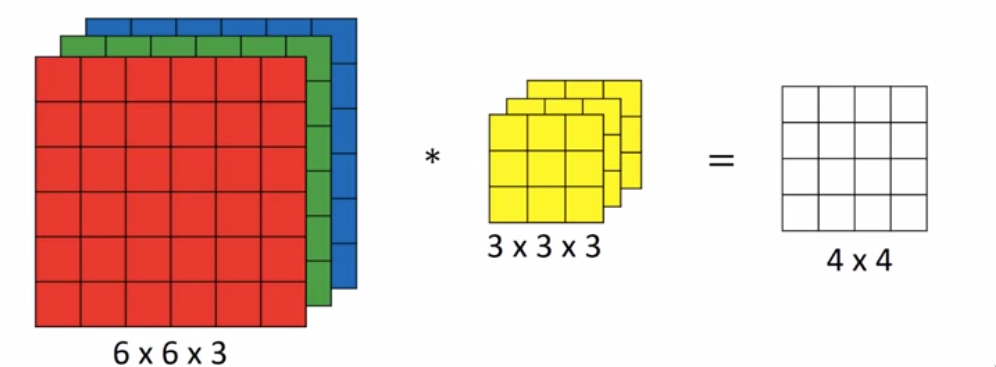
\includegraphics[scale=.5]{images/cnn-filter-volume.png}

Essentially the same as convolution over a 2D matrix. The number of channels
in the filter and the image have to be the same (3 in this case).

Multiple filters can be used by convolving the input image with each filter and then stacking
all the output images together. For example, given two filters and one input image,
the output matrix size will be 4x4x2, because there are two different filtered 2D output
matrices.

\subsection{One layer of a cnn}

Recall from forward prop:
\begin{gather*}
    Z^{[1]} = W^{[1]} A^{[0]} + \bm b^{[1]}\\
    A^{[1]} = g(Z^{[1]})
\end{gather*}

where $A^{[0]}$ is analogous to $X$. The input 6x6x3 image is $X$, the filter is $W$,
$\bm b$ is added to the output 4x4 matrix (element wise) which becomes $Z$, and then some
activation function $g$ is applied to that $Z$, giving the current layer's $A$. The number
of filters can be seen as the number of features.

\subsection{Cnn notation}

Superscript $[l]$ means relating to layer $l$.

$f^{[l]}$ = filter size ($f \times f$)

$p^{[l]}$ = padding thickness

$s^{[l]}$ = stride

Input dimensions are $n_H^{[l-1]} \times n_W^{[l-1]} \times n_c^{[l-1]}$.

Output dimensions are $n_H^{[l]} \times n_W^{[l]} \times n_c^{[l]}$.

$n^{[l]}$ = $\frac{n^{[l-1]}+2p^{[l]}-f^{[l]}}{s^{[l]}} + 1$, which is applicable to $n_H$ and $n_W$.

Each filter is $f^{[l]} \times f^{[l]} \times n_c^{[l-1]}$

Activations $a^{[l]}$ are $n_H^{[l]} \times n_W^{[l]} \times n_c^{[l]}$.

Vectorized: $A^{[l]}$ = $m \times n_H^{[l]} \times n_W^{[l]} \times n_c^{[l]}$

Weights $w^{[l]}$ are $f^{[l]} \times f^{[l]} \times n_c^{[l-1]}$

Vectorized: $W^{[l]}$ = $f^{[l]} \times f^{[l]} \times n_c^{[l-1]} \times n_c^{[l]}$

Bias $\bm b$ is just a vector of length $n_c^{[l]}$, though it becomes more convenient
to represent it as $1 \times 1 \times 1 \times n_c^{[l]}$ later.

\subsection{Example cnn (not vectorized)}

Input image $39 \times 39 \times 3$, first layer uses a set of 10 $3 \times 3$ filters,
second layer uses a set of 20 $5 \times 5$ filters, third layer uses 40 $5 \times 5$
filters. All layers use no padding, and stride is chosen arbitrarily.

Input image is $39 \times 39 \times 3$, so $n_W^{[0]}$ = $n_H^{[0]} = 39$
and $n_c^{[0]} = 3$.

For first layer, $f^{[1]}$ = 3, $s^{[1]}$ = 1, $p^{[1]}$ = 0. Because there are 10 filters,
there will be 10 channels in the first layer output, or $n_c^{[1]}$ = 10, and the dimensions
of a single channel in the first layer's output is calculated with $n^{[l]}$ =
$\frac{n^{[l-1]}+2p^{[l]}-f^{[l]}}{s^{[l]}} + 1$, which gives 37 for both width and height.
The activations will then be $37 \times 37 \times 10$.

For the second layer, $f^{[2]}$ = 5, $s^{[2]}$ = 2, $p^{[2]}$ = 0, $n_c^{[2]}$ = 20. The
output volume will then have dimensions of $17 \times 17 \times 20$, where 17 comes from
the $n_W$ and $n_H$ calculation and $20$ is $n_c$.

For the third layer, $f^{[3]}$ = 5, $s^{[2]}$ = 2, $p^{[2]}$ = 0. The output volume
then has dimensions of $7 \times 7 \times 40$.

After the last layer of filters has been processed, flatten out the final output volume
(in this case the $7 \times 7 \times 40$ volume) and feed it to a logistic/softmax regression.

A general trend is that the width and height of each channel in a volume of some layer will
be smaller than the previous layer's, while the number of channels increases as the layers go on.

\subsection{Pooling layers}

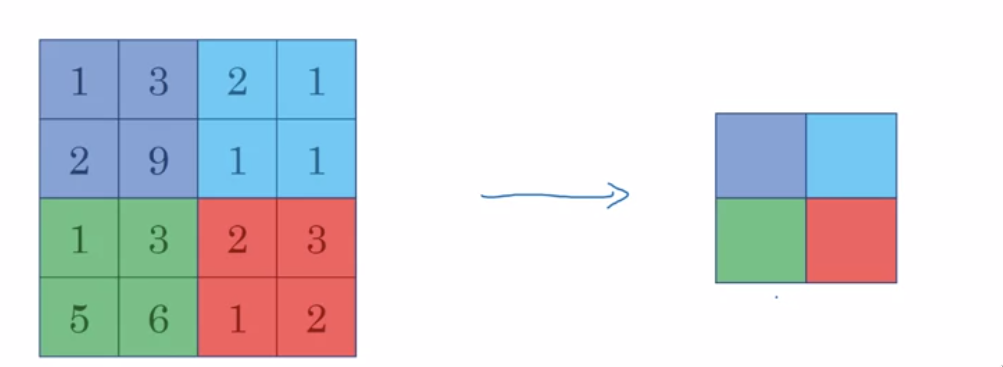
\includegraphics[scale=.5]{images/max-pooling.png}

Max pooling takes the largest number in each shaded region and puts it in the corresponding
color in the resulting $2 \times 2$ matrix. The hyperparameters can be represented as $f$ = 2,
$s$ = 2.

Max pooling can be helpful because it identifies important features in an image while also
reducing its size, which is computationally less expensive when running the cnn.

Average pooling takes the average of all the values in each shaded region instead of the
largest.

In pooling layers, there are no parameters to learn, the only parameters a pooling layer
has is its hyperparameters $f$ and $s$.

Convolutional and pooling layers are usually grouped together into a single layer because
the pooling layer has no parameters to learn.

\subsection{Fully connected layer}

A fully connected layer is just a regular deepnn layer. $W$ dimensions $n^{[l]} \times n^{[l-1]}$,
$\bm b$ dimensions $n^{[l]}$.

\subsection{Why convolutions}

Each filter only needs to learn its own parameters, and then can be applied anywhere on the
data (for example, in edge detection, a vertical edge filter is able to detect vertical edges
anywhere on the image after only learning a few parameters.

Each output depends on less inputs compared to a normal neural network, which improves
performance.

\subsection{Forward prop}

$e$th example, $n$th layer $l$ channel, $j$th layer $l-1$ channel
\begin{gather*}
    Z^{[l]}_{en} = \sum_{c=0}^{n_c^{[l-1]}}\text{convolve}(A^{[l-1]}_{ec},W^{[l]}_{cn}) + \bm b^{[l]}_n\\
    A^{[l]} = g(Z^{[l]})
\end{gather*}

$A^l$ and $Z^l$ have dimensions $m \times n_c^l \times n_h^l \times n_w^l$

$P^l$ is the pooled $A^l$ with dimensions $m \times n_c^l \times n^l_{ph} \times n^l_{pw}$,
and is equal to $A^l$ if there is no pooling.

$F^l$ is the flattened $P^l$ with length $m n_c^l n_{ph}^l n_{pw}^l$

$W^l$ is the weights for the filters in layer $l$ with dimensions $n_c^l \times n_c^{l-1}
\times f_H^l \times f_W^l$.

$0 \le e \le m$

$0 \le n \le n_c^l$

$0 \le u \le n_H^l$

$0 \le v \le n_W^l$

$n_{ph}^l = n_H^l/p^l_H$

$n_{pw}^l = n_W^l/p^l_W$

$p^l_H$ = pooling height in layer $l$

$p^l_W$ = pooling width in layer $l$

$0 \le c \le n_c^{l-1}$

$0 \le p \le f_H^l$

$0 \le q \le f_W^l$

$0 \le r \le n^{l-1}_{ph}$

$0 \le s \le n^{l-1}_{pw}$

Assume that all pooling layers use max pooling, and that the last layer $L$ is a dense layer with
a single softmax neuron.

\subsection{Back prop: $\frac{dL}{db}$}

Using chain rule:
\begin{gather*}
    \frac{dL}{db^l_n} = \sum_{u=0}^{n_H^l} \sum_{v=0}^{n_W^l}
                        \frac{dL}{dZ^l_{enuv}} \frac{dZ^l_{enuv}}{db^l_n}\\
    \frac{dL}{dZ^l_{enuv}} = \frac{dL}{dA^l_{enuv}} \frac{dA^l_{enuv}}{db^l_n}
\end{gather*}

\subsubsection{$\frac{dL}{dA^l_{enuv}}$}

\textbf{If $A^l_{enuv}$ is the max out of the elements in its pool, or there is no pooling layer:}

$P^l_{enyx} = A^l_{enu_{max}v_{max}}$, where $x = \floor(v_{max}/p_{W})$, $y = \floor(u_{max}/p_H)$
\[ \frac{dL}{dA^l_{enuv}} = \frac{dL}{dA^l_{enu_{max}v_{max}}} = \frac{dL}{dP^l_{enyx}} \]

$F^l_k = P^l_{enyx}$, where $k = (n_c^l n_{pm}^l n_{pw}^l)e + (n_{ph}^l n_{pw}^l) n + n_{pw}^l y + x$
\[ \cdots = \frac{dL}{dP^l_{enyx}} = \frac{dL}{dF^l_k} \]

Since $\frac{dL}{dA^l_{enu_{max}v_{max}}}$ = $\frac{dL}{dF_k}$, it might be helpful to calculate
$\frac{dL}{dF_k}$:
\[ \frac{dL}{dF^l_k} = \sum_{e=0}^m \sum_{i=0}^{n^L} \frac{dL}{dZ^L_{ei}} \frac{dZ^L_{ei}}{dF^l_k} \]

From $Z^L_{ei} = \sum_{j=0}^{k_{max}} (W^L_{ij} F^l_j) + \bm b_i$:
\begin{gather*}
    \frac{dZ_{ei}}{dF^l_k} = W_{ik}\\
    \frac{dL}{dF^l_k} = \sum_{e=0}^m \sum_{i=0}^{n^L} \frac{dL}{dZ^L_{ei}} W_{ik}
\end{gather*}

With $\frac{dL}{dF^l_k}$ solved, it is now possible to solve for $\frac{dL}{dA^l_{enuv}}$ in
the case that $dA^l_{enuv}$ is the largest in its pool.
\begin{gather*}
    \frac{dL}{dF^l} = W^{l T} \cdot \frac{dL}{dZ^L}\\
    \frac{dL}{dP^l} = \frac{dL}{dF^l}\text{.reshape}(P^l\text{.shape})
\end{gather*}

\textbf{If $A^l_{enuv}$ is not the largest in its pool:}

This part is not applicable for when there is no pooling done.

Because $P$ only holds the maximum value in each pool for $A$, changes in $A^l_{enuv}$ when $A^l_{enuv}$
is not the largest value will not affect $dL/dP$ and therefore $dL/dA$, which gives
\[
    \frac{dL}{dA^l_{enuv}} =
    \left\{\begin{array}{@{}l@{}}
            \frac{dL}{dP^l_{enyx}} \text{ if $A^l_{enuv}$ is the largest in its pool}\\
            0 \text{ otherwise}
    \end{array}\right.\,
\]

\textbf{Calculating $\frac{dL}{dA^l_{enuv}}$ (Conv $\rightarrow$ dense)}

In forward propagation, cache $n$, $u_{max}$, and $v_{max}$ into some array $I$ with the same
shape as $P^l$, which can be accessed with $I[n][y][x] = \begin{bmatrix}u_{max}\\v_{max}
\end{bmatrix}$.

Calculate $\frac{dL}{dP^l}$ using
\begin{gather*}
    \frac{dL}{dF^l} = W^{l T} \cdot \frac{dL}{dZ^L}\\
    \frac{dL}{dP^l} = \frac{dL}{dF^l}\text{.reshape}(P^l\text{.shape})
\end{gather*}

and then iterate over all inputs to $\frac{dL}{dP^l}$ ($n$, $y$, $x$) and use
\[ \frac{dL}{dA^l_{enu_{max}v_{max}}} = \frac{dL}{dP^l_{enyx}} \]

where $u_{max}$ and $v_{max}$ are fetched from $I[n][y][x]$.

For every $u \ne u_{max}$ and $v \ne v_{max}$, set $\frac{dL}{dA^l_{enuv}}$ to 0.

\textbf{Calculating $\frac{dL}{dA^l_{enuv}}$ (Conv $\rightarrow$ conv)}

Calculate $\frac{dL}{dP^l_{enyx}}$ using
\[ \frac{dL}{dP^l_{ecrs}} = \sum_{n=0}^{n_c^l} \sum_{u=0}^{n_H^l} \sum_{v=0}^{n_W^l}
\frac{dL}{dZ^{l+1}_{enuv}} \frac{dZ^{l+1}_{enuv}}{dP^l_{ecrs}} \]

Only $\frac{dZ^{l+1}_{enuv}}{dP^l_{ecrs}}$ needs to be calculated because $\frac{dL}{dZ^{l+1}_{enuv}}$
has already been calculated and should have been cached.

For any $n, u, v$, there is a 3D region of $P^l_{ecrs}$ contributing to $Z^{l+1}_{enuv}$, and
$\frac{dZ^{l+1}_{enuv}}{dP^{l}_{ecrs}} = W^{l+1}_{ncpq}$, where $p = r-u, q = s-v$ and $r = u
\cdots u+4, s = v \cdots v + 4$.

$\frac{dZ^{l+1}_{enuv}}{dP^{l}_{ecrs}}$ has shape $c_{max} \times r_{max} \times s_{max}
\times n_{max} \times u_{max} \times v_{max}$.

$\frac{dZ^{l+1}_{enuv}}{dP^{l}_{ecrs}}$ can be calculated in forward prop with
\[ \frac{dZ^{l+1}_{enuv}}{dP^l_{e,0\cdots n^{l+1}_c,0\cdots f_H^{l+1},0 \cdots f_W^{l+1}}}
= W^{l+1}\]

\[ \frac{dL}{dP^{l}} = \sum_{e=0}^m \sum_{n=0}^{n_c^{l+1}} \sum_{u=0}^{n_H^{l+1}} \sum_{v=0}^{n_W^{l+1}}
\frac{dL}{dZ^{l+1}_{enuv}} \frac{dZ^{l+1}_{enuv}}{dP^{l}_{ecrs}} \]

During forward prop, cache $(c, i_{max}, j_{max})$ at which $A^l_{ci_{max}j_{max}}$ is the maximum
in its pool.
\[ I^l[n,r,s] = \begin{bmatrix}i_{max}\\j_{max}\end{bmatrix} \]

where $r_{max} = i_{max}/2, s = j_{max}/2$.

$\frac{dL}{dA^{l}_{ecij}}$ can then be calculated with
\[ \frac{dL}{dA^l_{eci_{max}j_{max}}} = \frac{dL}{dP^l_{ecrs}} \]

where $(c,r,s)$ are all iterated over for all their possible values, and $i_{max}, j_{max}$
are obtained from $I^l[c,r,s]$.

$\frac{dL}{dZ^l_{ecij}}$ can then be determined:
\[ \frac{dL}{dZ^l_{ecij}} = \frac{dL}{dA^l_{ecij}} \frac{dA^l_{ecij}}{dZ^l_{ecij}} \]

$\frac{dL}{dA^l}$ was calculated earlier, and $\frac{dA}{dZ}$ is just the activation function derivative of $Z$.

From $z = wa + b$, $\frac{dZ^l_{ecij}}{db^l_c} = 1$.

$\frac{dL}{db^l_c}$ can then be represented as
\[ \frac{dL}{db^l_c} = \sum_{i=0}^{n_H^l} \sum_{j=0}^{n_W^l} \frac{dL}{dA^l_{ecij}} \frac{dA^l_{ecij}}{dZ^l_{ecij}} \]

\subsubsection{$\frac{dA^l_{enuv}}{dZ^l_{enuv}}$}

\begin{gather*}
    A = g(Z)\\
    \frac{dA^l_{enuv}}{dZ^l_{enuv}} = g'(Z^l_{enuv})
\end{gather*}

\subsubsection{$\frac{dZ^l_{enuv}}{db^l_n}$}

From $Z = \text{convolve}(P^{l-1},W^l) + b^l$ in forward prop:
\[ \frac{dZ^l_{enuv}}{db^l_n} = 1 \]

\subsection{Back prop: $\frac{dL}{dW}$}

\textbf{For conv $\rightarrow$ dense:}

\[ \frac{dL}{dW^l_{ncpq}} = \sum_{u=0}^{n_H^l} \sum_{v=0}^{n_W^l} \frac{dL}{dZ^l_{enuv}}
\frac{dZ^l_{enuv}}{dW^l_{ncpq}} \]

From $Z^l = \text{convolve}(P^{l-1},W^l) + b^l$
\[ \frac{dZ^l_{enuv}}{dW^l_{ncpq}} = P^{l-1}_{c,p+u,q+v} \]

Substituted:
\[ \frac{dL}{dW^l_{ncpq}} = \sum_{u=0}^{n_H^l} \sum_{v=0}^{n_W^l} \frac{dL}{dZ^l_{enuv}}
P^{l-1}_{c,p+u,q+v} \]

\textbf{For conv $\rightarrow$ conv:}

Similar to conv to dense, except $\frac{dZ^l_{ecij}}{dW^l_{ncgh}} = A^{l-1}_{c,g+i,h+j}$.

\subsection{Back prop summary}

Structure: Conv 1 $\rightarrow$ Conv 2 $\rightarrow$ Dense

\subsubsection{db: conv 1 $\rightarrow$ conv 2}
$l$ = 1

$0 \le e < m$

$0 \le c < n^l_c$

$0 \le i < n_H^l$

$0 \le j < n^l_W$

$0 \le r < n_H^l/p_H^l$

$0 \le s < n_W^l/p_W^l$

$p_W^l$ = pooling window width

$p_H^l$ = pooling window height

\begin{gather*}
    \frac{dL}{db^l_c} = \sum_{i=0}^{n^l_H} \sum_{j=0}^{n_W^l} \frac{dL}{dA^l_{ecij}}
    \frac{dA^l_{ecij}}{dZ^l_{ecij}}\\
    \frac{dL}{dA^l_{ec I^l[c,r,s].i_{max} I^l[c,r,s].j_{max}}} = \frac{dL}{dP^l_{ecrs}}\\
    \frac{dL}{dA^l_{ec i_{\text{not max}} j_{\text{not max}}}} = 0\\
    I^l[c,r,s] = \begin{bmatrix}i_{max}\\j_{max}\end{bmatrix}\\
    \frac{dA^l_{ecij}}{dZ^l_{ecij}} = g'(Z^l_{ecij})
\end{gather*}

$I$ is determined during forward prop.

\subsubsection{db: conv 2 $\rightarrow$ dense}
$l$ = 2

$0 \le e < m$

$0 \le n < n_c^l$

$0 \le u < n_H^l$

$0 \le v < n_W^l$

$y = u_{max}/p^l_H$

$x = v_{max}/p^l_W$

$p_W^l$ = pooling window width

$p_H^l$ = pooling window height

\begin{gather*}
    \frac{dL}{db^l_n} = \sum_{e=0}^m \sum_{u=0}^{n_H^l} \sum_{v=0}^{n_W^l} \frac{dL}{dZ^l_{enuv}}\\
    \frac{dL}{dZ^l_{enuv}} = \frac{dL}{dA^l_{enuv}} \frac{dA^l_{enuv}}{dZ^l_{enuv}}\\
    \frac{dL}{dA^l_{enuv}} = \left\{\begin{array}{@{}l@{}}
            \frac{dL}{dP^l_{enyx}} \text{ if $A^l_{enuv}$ is the largest in its pool}\\
            0 \text{ otherwise}
    \end{array}\right.\,\\
    \frac{dL}{dP^l} = \frac{dL}{dF^l}.\text{reshape}(P^l.\text{shape})\\
    \frac{dL}{dF^l} = W^{l,T} \frac{dL}{dZ^L}\\
    \frac{dA^l_{enuv}}{dZ^l_{enuv}} = g'(Z^l_{enuv})
\end{gather*}

\subsubsection{dw: conv 1 $\rightarrow$ conv 2}
$l = 1$

$0 \le n < n_c^l$

$0 \le c < n_c^{l-1}$

$0 \le p < f_H^l$

$0 \le q < f_W^l$

$0 \le u < n_H^l$

$0 \le v < n_W^l$

\begin{gather*}
    \frac{dL}{dW^l_{ncpq}} = \sum_{e=0}^m \sum_{u=0}^{n_H^l} \sum_{v=0}^{n_W^l} \frac{dL}{dZ^l_{enuv}}
    \frac{dZ^l_{enuv}}{dW^l_{ncpq}}\\
    \frac{dZ^l_{enuv}}{dW^l_{ncpq}} = P^{l-1}_{c,p+u,q+v}\\
\end{gather*}

\subsubsection{dw: conv 2 $\rightarrow$ dense}
$l = 2$

$0 \le n < n_c^l$

$0 \le c < n_c^{l-1}$

$0 \le g < f_H^l$

$0 \le h < f_W^l$

$0 \le u < n_H^l$

$0 \le v < n_W^l$

\begin{gather*}
    \frac{dL}{dW^l_{ncgh}} = \sum_{e=0}^m \sum_{u=0}^{n_H^l} \sum_{v=0}^{n_W^l} \frac{dL}{dZ^l_{enuv}}
    \frac{dZ^l_{enuv}}{dW^l_{ncgh}}\\
    \frac{dZ^l_{enuv}}{dW^l_{ncgh}} = A^{l-1}_{c,g+i,h+j}\\
\end{gather*}

\end{document}
